\documentclass[12pt]{article}
\usepackage{setspace,graphicx,amsmath,geometry,fontspec,titlesec,soul,bm,subfigure}
\titleformat{\section}[block]{\LARGE\bfseries}{\arabic{section}}{1em}{}[]
\titleformat{\subsection}[block]{\Large\bfseries\mdseries}{\arabic{section}.\arabic{subsection}}{1em}{}[]
\titleformat{\subsubsection}[block]{\normalsize\bfseries}{\arabic{subsection}-\alph{subsubsection}}{1em}{}[]
\titleformat{\paragraph}[block]{\small\bfseries}{[\arabic{paragraph}]}{1em}{}[]
\setmainfont{Times New Roman}
\renewcommand{\baselinestretch}{1.15}
\renewcommand\contentsname{Inhaltverzeichnis}
\geometry{a4paper,left=2.5cm,right=2.5cm,top=2.5cm,bottom=2.5cm}
\begin{document}
	\newpagestyle{main}{            
		\sethead{Ziqing Yu}{Ingenieurgeodäsie Übung 3}{3218051}     
		\setfoot{}{\thepage}{}     
		\headrule                                     
		\footrule                                       
	}
	\pagestyle{main}
\tableofcontents
\newpage
\section{Einleitung}
In dieser Übung wird eine Entwurfsplanung mit Längsprofil von einem Abschnitt einer regionalen Straßenverbindung gezeichnet. Die Trasse behaltet 2 Geraden, 2 Klothoiden und 1 Kreisbogen. Anschlussgeraden, Entwurfsgeschwindigkeit, Fahrbahnbreite, Querneigung, Reibungswert, und A Parameter Klothoide sind gegeben. Die Koordinaten von Haupt- und Zwischenpunkten sollen auch dokumentiert werden. 
\newpage
\section{Trassierungsparameter, Koordinaten und Länge}
Entwurfsgeschwindigkeit, Querneigung, Reibungsbeiwert, A Parameter der Klothoide sind bekannt.
\begin{gather*}
V_e  = 70 km/h = 19,44m/s \\
q = 6\% \\
fr = 0,4 \\ 
A = 150m 
\end{gather*}
Mit obigen Parametern ist der mindeste Radius zu bestimmen
\begin{gather*}
R > \frac{(1 - fr \cdot q) \cdot V_e^2}{(q + fr) \cdot g} \Rightarrow R > 81,857m \\
R > \frac{V_e^2}{(0,85m/s^2 + g \cdot q)} \Rightarrow R > 262,925m 
\end{gather*}
In dieser Aufgabe nehme ich $R = 350 m$, dann sind Klothoidelänge $L = \frac{A^2}{R} = 64,286m$ und Tangentenwinkel $\tau = \frac{L}{2R} = 0,0918 rad$ \newline
\begin{figure*}[ht]\centering
	\subfigure[Klothoid]{
		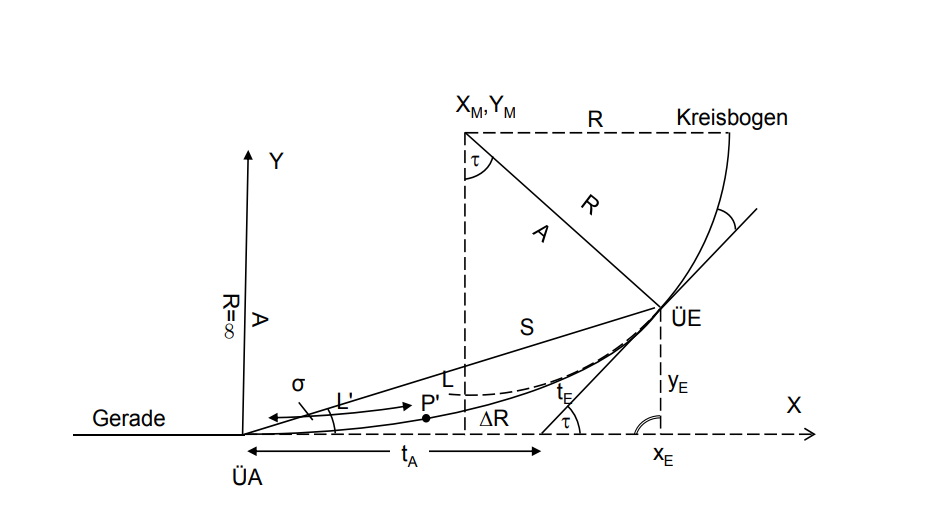
\includegraphics[width=0.9\textwidth]{klotoid.png}}
\end{figure*}
In diesem Graph ist Koordinate von ÜA $(0,0)$, um die Koordinate von ÜE zu rechnen, sind folgende Formeln zu nutzen:
\begin{gather*}
l = \frac{L}{A} = 0,4268\\
x_{UE} = (l - \frac{l^5}{40} + \frac{l^9}{3456}) \cdot A = 64,232m\\
y_{UE} = (\frac{l^3}{6} - \frac{l^7}{336} + \frac{l^{11}}{42240}) \cdot A =  1,967m
\end{gather*}
Danach haben wir
\begin{gather*}
t_A = x_{UE} - \frac{y_{UE}}{\tan \tau} = 42,876m \\
t_E = \sqrt{(x_{UE} - t_A)^2 + y_{UE}^2} = 21,446m \\
\Delta R = y_{UE} - R \cdot (1 - \cos (\tau)) = 0,4918 m 
\end{gather*}
Die Länge zwischen ÜA und Lotpunkt $x_{lot} = x_{UE} - R \cdot \sin(\tau) = 32,134m$ \newline
\newline
Alle der obigen Parametern sollen in die lokalen Koordinatensystem transformiert werden. \newline
Richtungswinkel von beiden Geraden:
\begin{gather*}
t_{5152} = \arctan(\frac{y_{52} - y_{51}}{x_{51} - x{51}}) = 5,6712 rad\\
t_{6162} = \arctan(\frac{y_{62} - y_{61}}{x_{61} - x{61}}) = 3,2745 rad
\end{gather*}
Schnittwinkel der beiden Geraden $\alpha =´2 \pi - (t_{5152} - (t_{6162} + \pi)) = 0,7449rad$, der Schnittpunkt von beiden Geraden kann man rechnen oder in AutoCAD lesen: $x_{schnitt} = 2189,778m,\ \ y_{schnitt} = 694,664m$. Die Länge zwischen Klothoidanfangspunkt und Schnittpunkt $S = x_{lot} + (R + \Delta R) \cdot \tan (\frac{\alpha}{2}) = 169,067m$ \newline
Mit polares Anhänge werden die Koordinaten von beiden Klotoidanfangspunkten berechnet.
\begin{gather*}
x_{a1} = x_{schnitt} + S \cdot cos(t_{5152}) = 2051,396m \\
y_{a1} = y_{schnitt} + S \cdot sin(t_{5152}) = 791,792m \\
x_{k1} = x_{a1} + t_a \cdot cos(t_{5152}) = 2086,490m \\
y_{k1} = y_{a1} + t_a \cdot sin(t_{5152}) = 767,160m \\
x_{e1} = x_{k1} + S \cdot cos(t_{5152} + \tau) = 2105,099m \\
y_{e1} = y_{k1} + S \cdot sin(t_{5152} + \tau) = 756,501m 
\end{gather*}
Analog für die andere Klothoid: 
\begin{gather*}
(x_{a2},y_{a2}) = (2357,353m, \ \ 717,069m) \\
(x_{e2},y_{e2}) = (2293,428m, \ \ 710,507m)
\end{gather*}
Die Länge der Geraden sind:
\begin{gather*}
L_{Gerade1} = \sqrt{(x_{51} - x_{a1})^2 + (y_{51} - y_{a1})^2} = 66,041m \\
L_{Gerade2} = \sqrt{(x_{62} - x_{a2})^2 + (y_{62} - y_{a2})^2} = 54,012m
\end{gather*}
Mittelpunkt der Kreisbogen ist auch mit polarem Anhängen zu bestimmen. 
\begin{gather*}
x_m = x_{e1} + R \cdot \cos (t_{5152} + \tau + \frac{\pi}{2}) \\
y_m = y_{e1} + R \cdot \sin (t_{5152} + \tau + \frac{\pi}{2}) \\
\end{gather*}
Winkel der Kreisbogen: 
\begin{equation*}
\beta = t_{e2m} - t_{e1m} = \arctan(\frac{y_m - y_{e2}}{x_m - x_{e2}}) - \arctan(\frac{y_m - y_{e1}}{x_m - x_{e1}}) = 0,5612 rad
\end{equation*}
Länge von Kreisbogen $L_{Kreisbogen} = 196,431m$\newline
Länge der Straße $L = L_{Gerade1} + L_{Gerade2} + L_{Klotoid} \cdot 2 + L_{Kreisbogen} = 445,055m$
\section{Zwischenpunkten und Zeichnung}
Alle Zwischenpunkten auf Klothoid werden analog wie Klothoidendpunkten gerechnet.
\begin{gather*}
l_z = \frac{L_z}{A}\\
x_{z} = (l_z - \frac{l_z^5}{40} + \frac{l_z^9}{3456}) \cdot A\\
y_{z} = (\frac{l_z^3}{6} - \frac{l_z^7}{336} + \frac{l_z^{11}}{42240}) \cdot A
\end{gather*}
hier ist $L_z = 20,40,60$, dann ist ein Transformation gemacht werden muss, für die erste Klotoid:
\begin{gather*}
\begin{bmatrix}
x_{zwischen} \\
y_{zwischen}
\end{bmatrix} = \begin{bmatrix}
\cos (t_{5152}) & -\sin (t_{5152}) \\
\sin (t_{5152}) & \cos (t_{5152})
\end{bmatrix} \cdot \begin{bmatrix}
x_z \\
y_z
\end{bmatrix} + \begin{bmatrix}
x_{a1} \\
y_{a1}
\end{bmatrix}
\end{gather*}
für die zweite Klothoid: 
\begin{gather*}
\begin{bmatrix}
x_{zwischen} \\
y_{zwischen}
\end{bmatrix} = \begin{bmatrix}
\cos (t_{6162} + \pi) & -\sin (t_{5152} + \pi)\\
\sin (t_{5152} + \pi)& \cos (t_{5152} + \pi)
\end{bmatrix} \cdot \begin{bmatrix}
x_z \\
y_z
\end{bmatrix} + \begin{bmatrix}
x_{a2} \\
y_{a2}
\end{bmatrix}
\end{gather*}
Die Zwischen Punkte in Kreisbogen werden automatisch von AutoCAD berechnen, die Koordinaten von allen Zwischenpunkten sind in  einer Tabelle in AutoCAD dokumentiert. 
\newpage 
\noindent Die Zeichnung der Trasse: 
\begin{figure*}[ht]\centering
	\subfigure[Abschnitt 5]{
		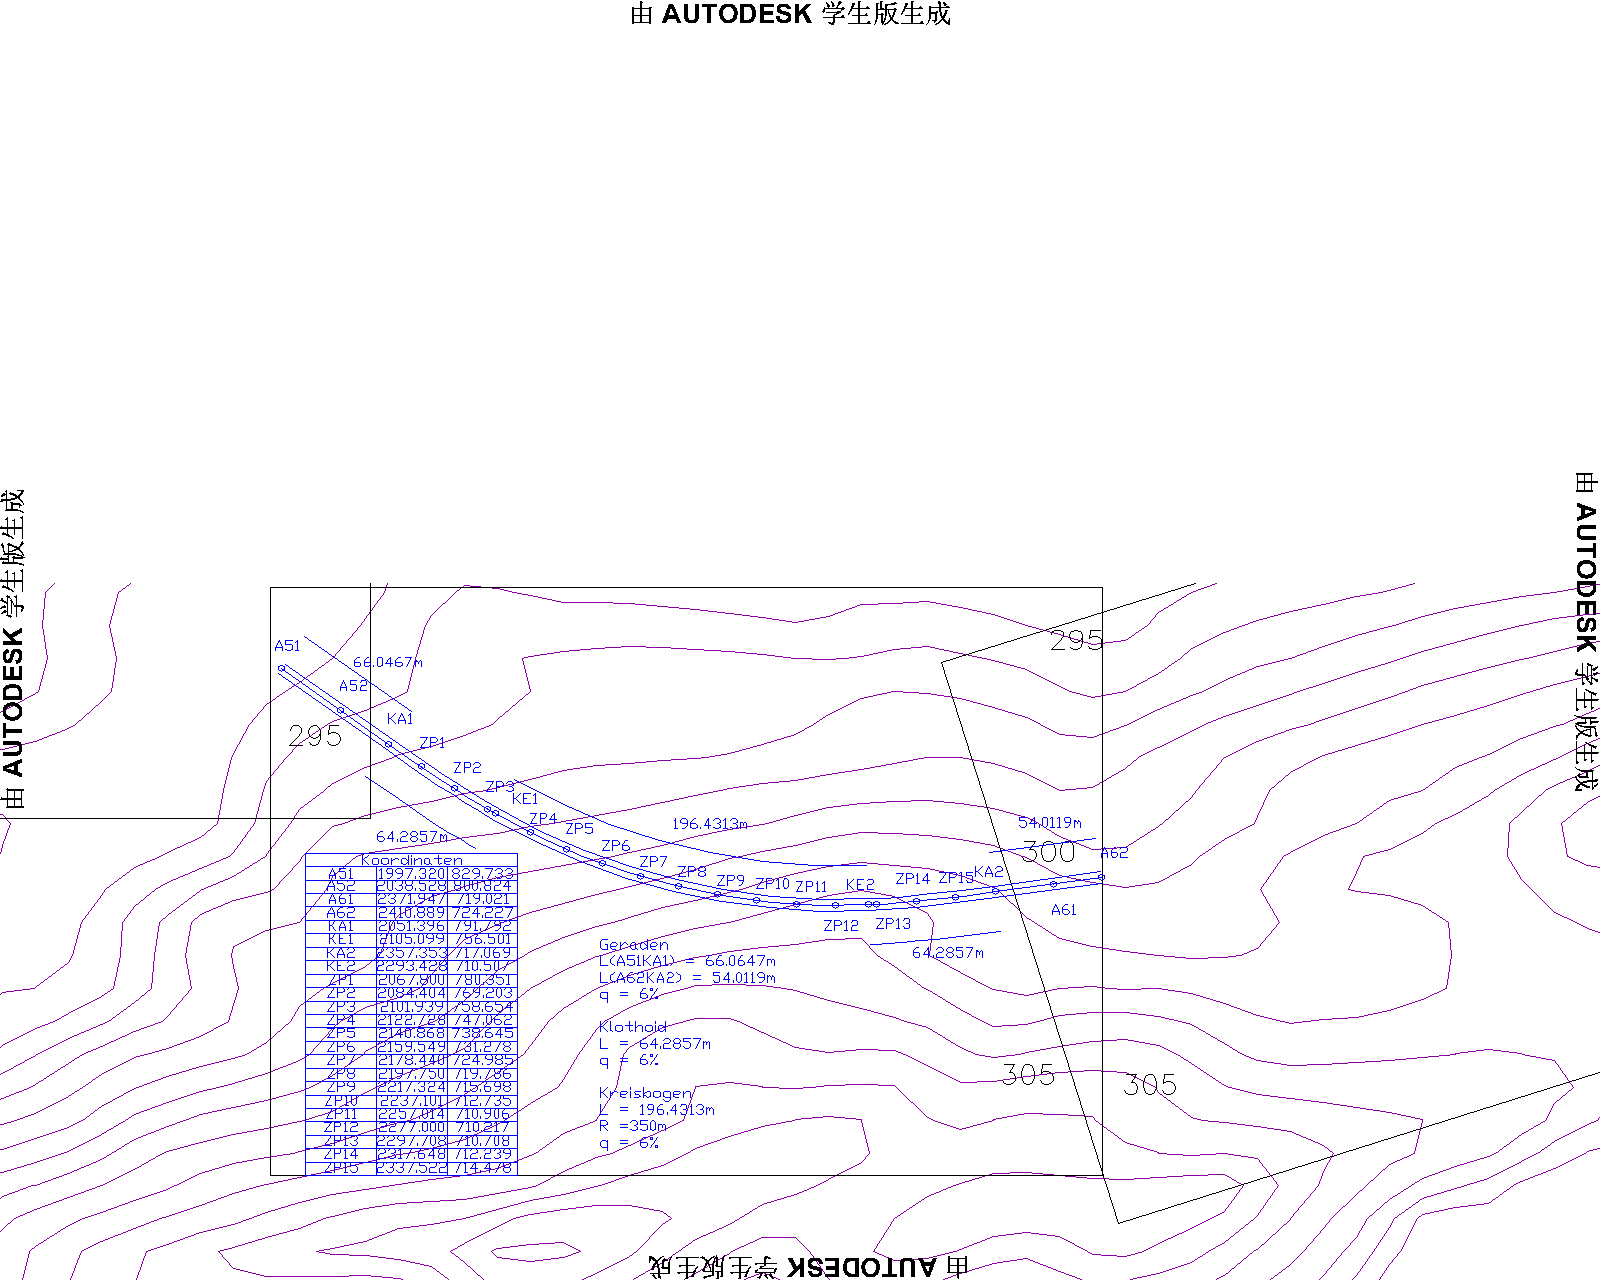
\includegraphics[width=0.5\textwidth]{zeichnung.png}}
\end{figure*}
\newline
Der A3 DIN Entwurfsplan ist per E-Mail geschickt. \newline
Längsprofil: 
\begin{figure*}[ht]\centering
	\subfigure[Längsprofil]{
		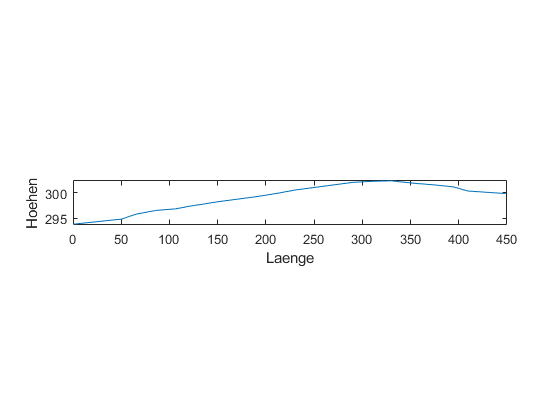
\includegraphics[width=0.8\textwidth]{langsprofil.png}}
\end{figure*}
\end{document}
